\documentclass{article}
\usepackage{algpseudocode}
\usepackage[ruled]{algorithm}
\usepackage{url}
\usepackage{framed}
\usepackage{amsfonts,amsmath,amsthm,amssymb}
\usepackage{graphicx}
\usepackage{url}
\usepackage{color}
\usepackage{geometry}

\geometry{margin=1.2in}

\newcommand {\mean} {\ensuremath {\mathop{\mathrm{mean}}}}
\newcommand {\median} {\ensuremath {\mathop{\mathrm{median}}}}
\newcommand {\N} {\ensuremath {\mathcal{N}}}
\newcommand {\IE} {\ensuremath {\mathbb{E}}}
\newcommand {\cov} {\ensuremath {\mathop{\mathrm{cov}}}}
\newcommand {\BEL} {\ensuremath {\mathop{\mathrm{BEL}}}}

\newtheorem{dfn}{Definition}
\newtheorem{thm}{Theorem}
\newtheorem{lmm}{Lemma}

\title{VOI-aware Monte Carlo Sampling in Trees}
\author {David Tolpin, Solomon Eyal Shimony \\
Department of Computer Science, \\
Ben-Gurion University of the Negev, Beer Sheva, Israel \\
\{tolpin,shimony\}@cs.bgu.ac.il}

\begin{document}

\maketitle

\begin{abstract}
Upper bounds for the VOI are provided for pure exploration in the
Multi-armed Bandit Problem. Sampling policies based on the upper
bounds are suggested. Empirical evaluation of the policies and
comparison to the UCB1 and UCT policies is provided
on random problem instances as well as on the Go game.
\end{abstract}


\section{Introduction and Definitions}

Taking a sequence of samples in order to minimize the
regret of a decision based on the samples is abstracted by the
{\em Multi-armed Bandit Problem.} In the Multi-armed Bandit problem
we have a set of $K$ arms. Each arm can be pulled multiple
times. When the $i$th arm is pulled, a random reward $X_i$ from an
unknown stationary distribution is returned.  The reward is bounded
between 0 and 1.

The simple regret of a sampling policy for the Multi-armed Bandit
Problem is the expected difference between the best expected reward
$\mu_*$ and the expected reward $\mu_j$ of the arm with the best sample mean
$\overline X_j=\max_i\overline X_i$:
\begin{equation}
\label{eqn:simple-regret}
\IE[R]=\sum_{j=1}^K\Delta_j\Pr(\overline X_j=\max_i\overline X_i)
\end{equation}
where $\Delta_j=\mu_*-\mu_j$.
Strategies that minimize the simple regret are called pure exploration
strategies \cite{Bubeck.pure}. Principles of rational metareasoning
\cite{Russell.right} suggest that at each step the arm with the great
value of information (VOI) must be pulled, and the sampling must be
stopped and a decision must be made when no arm has positive VOI. 

To estimate the VOI of pulling an arm, either a certain 
distribution of the rewards should be assumed (and updated based on
observed rewards), or a distribution-independent bound on the VOI can be
used as the VOI estimate. In this paper, we use {\em concentration inequalities}
to derive distribution-independent bounds on the VOI.

\section{Some Concentration Inequalities}

Let $X_1, \ldots, X_n$ be i.i.d. random variables with values from $[0,1]$,
$X=\frac 1 n \sum_{i=1}^n X_i$. Then 
\begin{description}
\item[Hoeffding's inequality \rm{\cite{Hoeffding.ineq}}:] 
\begin{equation}
\Pr(X-\IE[X] \ge a) \le \exp ( -2na^2)
\label{eqn:conc-hoeffding}
\end{equation}
\item[Empirical Bernstein's inequality
  \rm{\cite{MaurerPontil.benrstein}}:]\footnote{see
    Appendix~\ref{app:deriv-conc-empbernstein} for derivation}
\begin{eqnarray}
\Pr(X-\IE[X] \ge a) &\le& 2\exp \left( - \frac {na^2} {\frac {14} {3}
                          \frac {n} {n-1}a+2\overline\sigma_n^2}\right)\nonumber\\
                    &\le& 2\exp \left( - \frac {na^2} {10a+2\overline\sigma_n^2}\right)
\label{eqn:conc-empbernstein}
\end{eqnarray}
where sample variance $\overline\sigma_n^2$ is
\begin{equation}
\overline\sigma_n^2=\frac 1 {n(n-1)} \sum_{1\le i < j\le n}(X_i-X_j)^2
\label{eqn:sample-variance}
\end{equation}
\end{description}
Bounds (\ref{eqn:conc-hoeffding}, \ref{eqn:conc-empbernstein}) are symmetrical
around the mean. Bound~(\ref{eqn:conc-empbernstein}) is tighter than
(\ref{eqn:conc-hoeffding}) for small $a$ and $\overline\sigma_n^2$. 

\section{Upper Bounds on Value of Information}

The intrinsic VOI $\Lambda_i$ of pulling an arm is the expected decrease
in the regret compared to selecting an arm without pulling any arm at
all. The \textit{myopic} VOI estimate is of limited applicability to
Monte Carlo sampling, since the effect of a single sample is small,
and the myopic VOI estimate will often be non-positive, resulting in premature
termination of the search. However, $\Lambda_i$ can be estimated as the intrinsic 
value of perfect information $\Lambda_i^p$ about the mean reward of the $i$th arm. Two
cases are possible:
\begin{itemize}
\item the arm ($\alpha$) with the highest sample mean is pulled, and the 
mean of the arm is lower than the sample mean the second-best arm ($\beta$);
\item another arm is pulled, and the mean of the arm is higher
than the current highest sample mean ($\alpha$).
\end{itemize}
$\Lambda_i^p$ can be bounded from above as the probability that a
different arm is selected, multiplied by the
maximum possible increase in the reward:

\begin{thm} The intrinsic value of perfect information $\Lambda_i^p$ about the $i$th arm is
  bounded from above as
\begin{equation}
  \Lambda_i^p \le \left\{
  \begin{array}{l l}
    \Pr(\IE[X_i] \le \overline X_\beta)\overline X_\beta & \mbox{if $i=\alpha$} \\
    \Pr(\IE[X_i] \ge \overline X_\alpha)(1-\overline X_\alpha) & \mbox{otherwise}
  \end{array} \right.
\label{eqn:thm-vopi}
\end{equation}
\end{thm}

The search time is finite, and in a simple case the \textit{search
  budget} specified as the maximum number of samples.
An estimate based on the perfect intrinsic VOI does not take in
consideration the remaining number of samples. Given two arms
with the same intrinsic perfect VOI, the VOI
estimate of the arm pulled fewer times so far should be higher.

\begin{dfn} The \textbf{blinkered estimate} of intrinsic VOI information of the
  $i$th arm is the intrinsic VOI of pulling the $i$th arm for the
  remaining budget.
\end{dfn}

\begin{thm} Denote the current number of samples of the $i$th arm as
  $n_i$. The blinkered estimate $\Lambda_i^b$ of intrinsic value of
  information of pulling the $i$th arm for the remaining budget of $N$
  samples is bounded from above as
\begin{equation}
  \Lambda_i^b \le \left\{
  \begin{array}{l l}
    \Pr(\overline X_i'\le\overline X_\beta)\overline X_\beta\frac N {N+n_i} & \mbox{if $i=\alpha$} \\
    \Pr(\overline X_i'\ge\overline X_\alpha)(1-\overline  X_\alpha)\frac N {N+n_i} &  \mbox{otherwise}
  \end{array} \right.
\label{eqn:thm-be}
\end{equation}
where $\overline X_i'$ is the sample mean of the $i$th arm after $n_i+N$ 
samples.
\end{thm}

 The probabilities in equations (\ref{eqn:thm-vopi}, \ref{eqn:thm-be}) can be bounded from above using concentration
inequalities. In particular, Lemma~\ref{lemma:hoeffding-prob-bounds} is
based on the Hoeffding inequality (\ref{eqn:conc-hoeffding}):
\begin{lmm} The probabilities in equations (\ref{eqn:thm-vopi}, \ref{eqn:thm-be}) are bounded from above as
\begin{eqnarray}
\Pr(\IE[X_i] \le \overline X_\beta|i=\alpha)& \le & \exp(-2 (\overline X_i - \overline X_\beta)^2 n_i)\nonumber\\
\Pr(\IE[X_i] \ge \overline X_\alpha|i\ne\alpha)& \le & \exp(-2 (\overline X_\alpha - \overline X_i)^2 n_i)\nonumber\\
\Pr(\overline X_i' \le \overline X_\beta|i=\alpha)& \le &  2\exp\left(-\frac {2(\overline X_i - \overline X_\beta)^2  (n_i+N) n_i} {(\sqrt n_i + \sqrt {n_i + N})^2}  \right) < 2\exp\left(-\frac {(\overline X_i - \overline X_\beta)^2 n_i} 2 \right)\nonumber\\
\Pr(\overline X_i' \ge \overline X_\alpha|i\ne\alpha)& \le & 2\exp\left(-\frac {(\overline X_\alpha - \overline X_i)^2 (n_i+N) n_i} {(\sqrt n_i + \sqrt {n_i + N})^2} \right) <  2\exp\left(-\frac {(\overline X_\alpha - \overline X_i)^2 n_i} 2 \right)
\label{eqn:probound-perf-hoeffding}
\end{eqnarray}
\label{lemma:hoeffding-prob-bounds}
\end{lmm}

Better bounds can be obtained through tighter estimates on
the probabilities, for example, based on the empirical Bernstein
inequality (\ref{eqn:conc-empbernstein}) or through a more careful
application of the Hoeffding inequality (Appendix~\ref{app:better-hoeffding-bound}).

\section{VOI-based Sampling Control}

\subsection{Selection Criterion}

Following the principles of rational metareasoning, an arm with the highest upper bound $\hat
\Lambda$ on the perfect value of information should be pulled at each
step. This way, arms known to have a low VOI  would be pulled less frequently.

\subsection{Termination Condition}

The upper bounds~(\ref{eq:lambda-hoeffding-bounds}, \ref{eq:lambda-bernstein-bounds}) decrease exponentially with the
number of pulls $n$. When the upper bound of the VOI for all arms
becomes lower than a threshold $\lambda$, which can be chosen based on
resource constraints, the sampling should be stopped, and an arm should
be chosen.

\subsection{Sample Redistribution in Trees}

UCT forwards samples to the next search stage when the winner at the
current state is known with high confidence. VOI-based termination
condition can be used to stop the sampling in the current state early
and save the remaining samples for re-use in a later search state.

\section{Empirical Evaluation}

\subsection{Selecting The Best Arm}

Figure~\ref{fig:random-instances}

\begin{figure}[h]
\centering
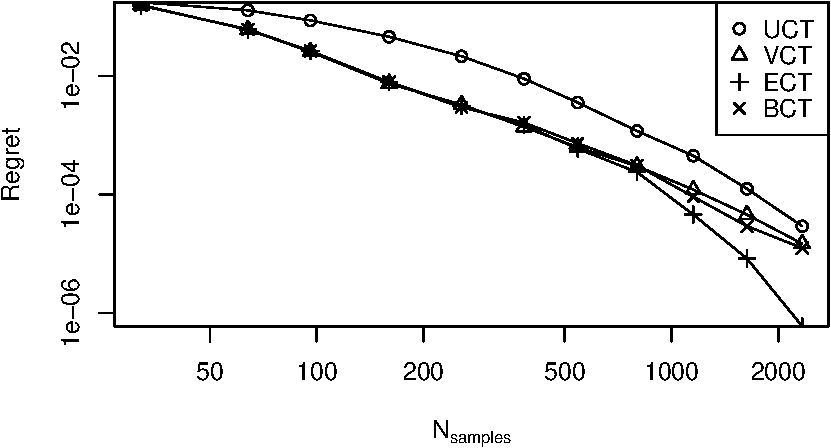
\includegraphics[scale=0.8]{flat.pdf}
\caption{Random instances: regret vs. number of samples}
\label{fig:random-instances}
\end{figure}


\subsection{Playing Go Against UCT}

Figure~\ref{fig:uct-against-vct}, Figure~\ref{fig:uct-against-ect}, Figure~\ref{fig:uct-against-bct},
Figure~\ref{fig:best-winning-rate}.

\begin{figure}[h]
\centering
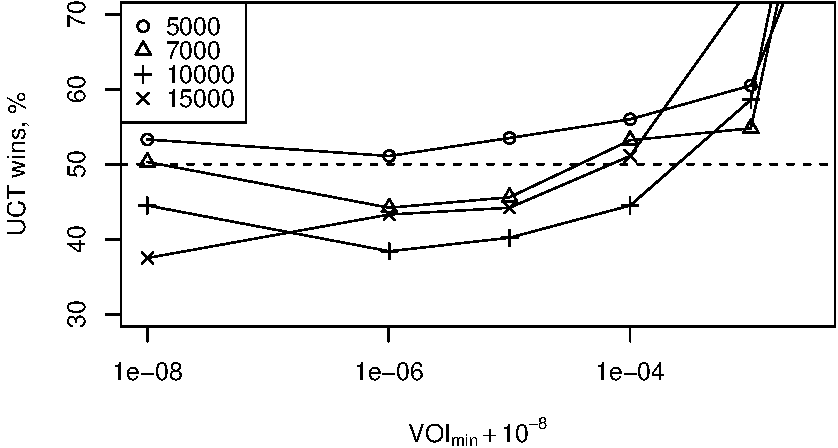
\includegraphics[scale=0.8]{vct-wins.pdf}
\caption{Go: winning rate --- UCT against VCT}
\label{fig:uct-against-vct}
\end{figure}

\begin{figure}[h]
\centering
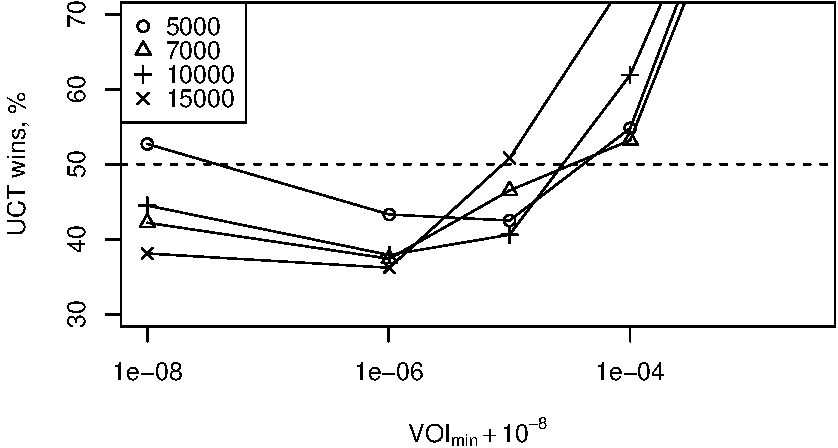
\includegraphics[scale=0.8]{ect-wins.pdf}
\caption{Go: winning rate --- UCT against ECT}
\label{fig:uct-against-ect}
\end{figure}

\begin{figure}[h]
\centering
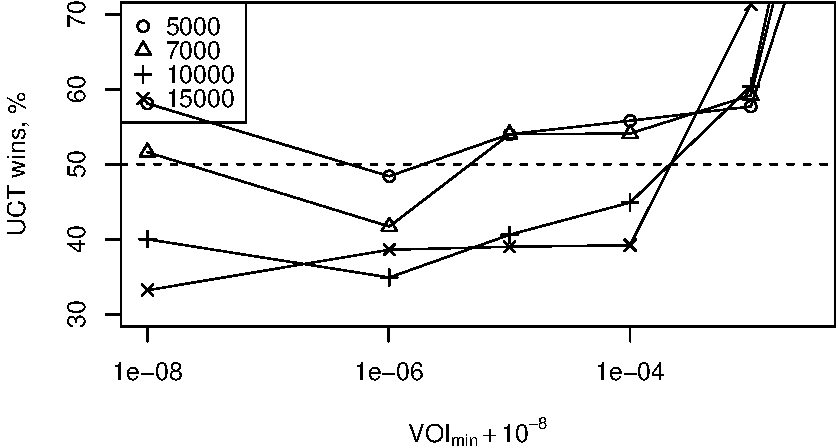
\includegraphics[scale=0.8]{bct-wins.pdf}
\caption{Go: winning rate --- UCT against BCT}
\label{fig:uct-against-bct}
\end{figure}

\begin{figure}[h]
\centering
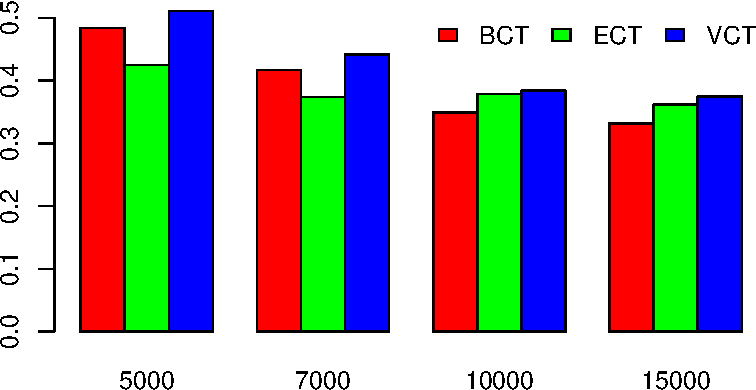
\includegraphics[scale=0.8]{bests-colorful.pdf}
\caption{Go: best winning rate comparison}
\label{fig:best-winning-rate}
\end{figure}

\clearpage

\appendix

\section{Empirical Bernstein Inequality}
\label{app:deriv-conc-empbernstein}

Theorem~4 in~\cite{MaurerPontil.benrstein} states that
\[\Pr\left(\IE[X]-\overline X_n \ge \sqrt { \frac {2\overline\sigma_n^2 \ln 2/\delta} n } + \frac {7 \ln 2/\delta} {3(n-1)}\right)\le \delta,\]
Therefore
\[\Pr\left(\IE[X]-\overline X_n \ge \sqrt { \left(\frac {7 \ln 2/\delta} {3(n-1)}\right)^2+\frac {2\overline\sigma_n^2 \ln 2/\delta} n } + \frac {7 \ln 2/\delta} {3(n-1)}\right)\le
\delta.\]
$a=\sqrt { \left(\frac {7 \ln 2/\delta} {3(n-1)}\right)^2+\frac {2\overline\sigma_n^2 \ln 2/\delta} n } + \frac {7 \ln 2/\delta} {3(n-1)}$ is a root of
square equation
\[a^2-a\frac {14 \ln 2/\delta} {3(n-1)} -\frac {2\overline\sigma_n^2 \ln 2/\delta} n=0\]
which, solved for $\delta\triangleq\Pr(\IE[X]-\overline X_n\ge a)$,
gives
\[\Pr(\IE[X]-\overline X_n\ge a)\le 2\exp \left( - \frac {na^2} {\frac {14} {3} \frac {n} {n-1}a+2\overline\sigma_n^2}\right)\]
Other derivations, giving slightly different results, are possible.

\section{Better Hoeffding-Based Bound on Value of Perfect Information}
\label{app:better-hoeffding-bound}

The bound can be supposedly be improved by selecting a midpoint
$0 < y < \overline X_\beta$ and computing the bound as the sum of two parts:
\begin{itemize}
\item $\overline X_\beta-y$ multiplied by the probability that
  $\mu_\alpha \le \overline X_\beta$;
\item $\overline X_\beta$ multiplied by the probability that $\mu_\alpha\le
  y$.
\end{itemize}.
\[ V_{\overline X=\overline X_\alpha} \le (\overline X_\beta-y)\exp\left(-2n(\overline X_\alpha-\overline X_\beta)^2\right)+\overline X_\beta\exp\left(-2n(\overline X_\alpha-y)^2\right) \]

\vspace{\baselineskip}

The minimum of $V^*$ is achieved when $\frac {dV^*} {dy}=0$, that
is, when $y$ is the root of the following equation:
\[ 4\overline X_\beta n(\overline X_\alpha-y)=\exp\left(-2n\left(\frac {\overline X_\alpha-\overline X_\beta}
    {\overline X_\alpha-y}\right)^2\right) \]
If a root in the interval  $0\le y\le\beta$ exists, then the
number of samples is bounded as
\[n\le\frac 1 {4\overline X_\beta(\overline X_\alpha-\overline X_\beta)}\]
by observing that the right-hand side 
is at most $1$ (a negative power), and the left-hand side is at least
$4\overline X_\beta n(\overline X_\alpha-\overline X_\beta)$.
So, the bound can supposedly be improved for smaller values of
$n$. The improvement is more significant when the current best and
second-best sample means are close.

The derivation for the other case
(sampling an item that can be better than the current best) is
obtained by substitution $1-\overline X, 1-\overline X_\alpha, 1-y$ instead of
$\overline X_\alpha, \overline X_\beta, y$:

\[ V_{\overline X\ne\overline X_\alpha} \le (y-\overline X_\alpha)\exp\left(-2n(\overline X_\alpha-\overline
  X)^2\right)+(1-\overline X_\alpha)\exp\left(-2n(y-\overline X)^2\right) \]

The anticipated influence of the improved
VOI estimate would be that the selected item will be a less discovered
one and further from the current best or second-best.

A closed-form solution for $y$ cannot be obtained, but given
$\overline X_\alpha, \overline X_\beta, n$, the value of $y$ can be efficiently
computed. It should be determined empirically whether the improved
estimate has justified influence on the performance of the algorithm.

\bibliographystyle{plain}
\bibliography{refs}

\end{document}
